\documentclass{beamer}

\usepackage{graphicx}
\usepackage{hyperref}

\usefonttheme{serif}

\title{1 - Binary and logic}
\author{}
\date{}

\begin{document}

\frame{\titlepage}

\begin{frame}
  \frametitle{Agenda}
  \tableofcontents
\end{frame}

\section{Inside the computer: power supply unit}

\begin{frame}
  \frametitle{Who's this? The power supply unit!}
  \begin{figure}
    \centering
    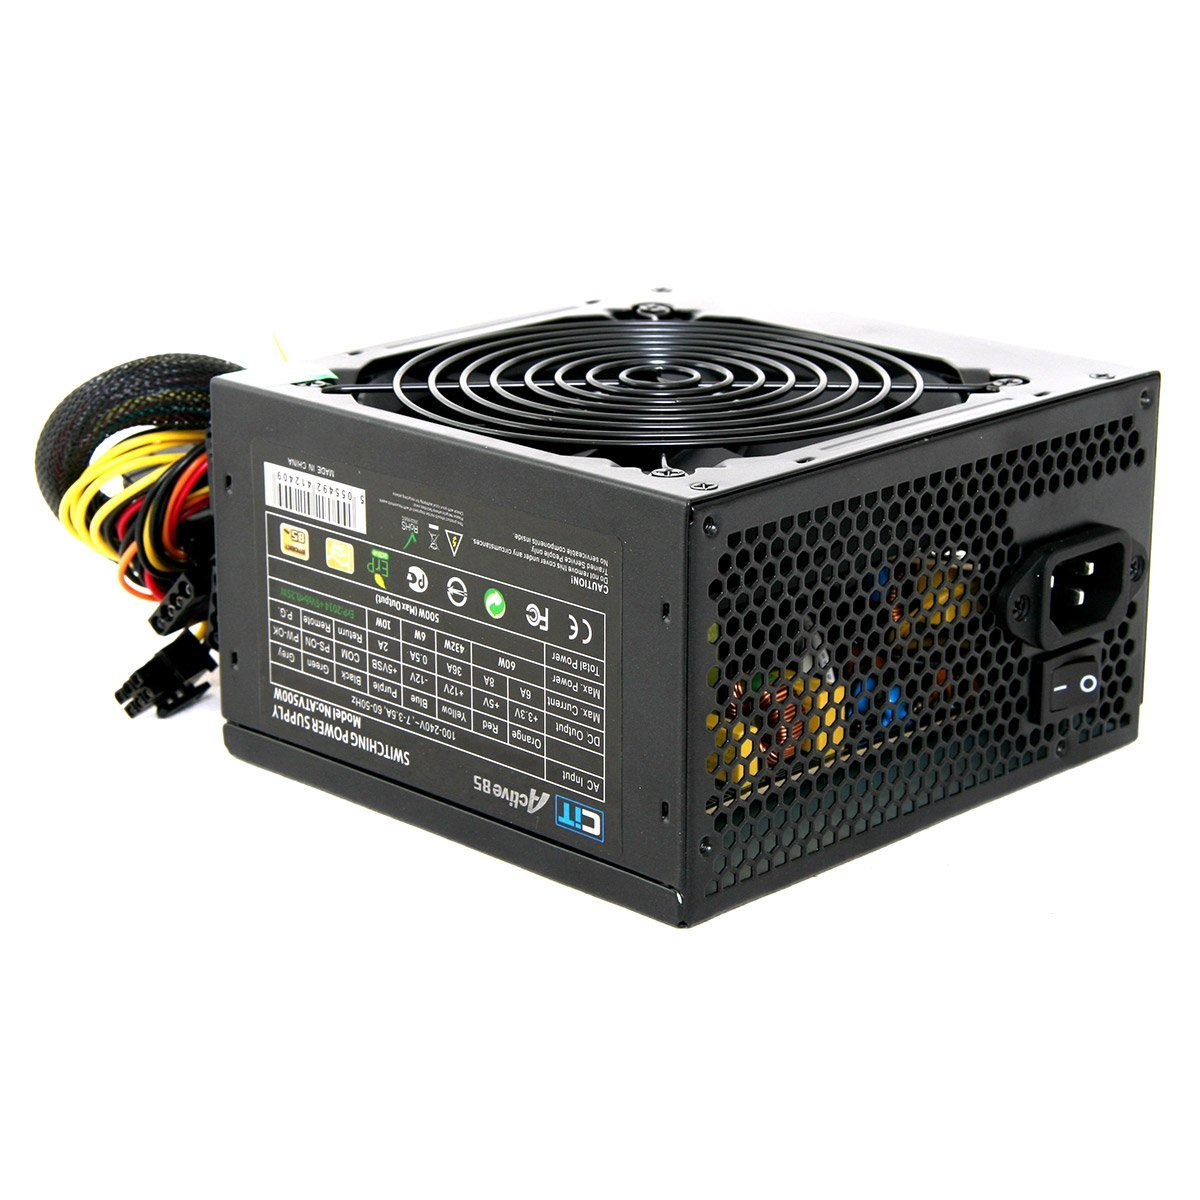
\includegraphics[width=0.4\textwidth]{res/psu.jpg} \\
    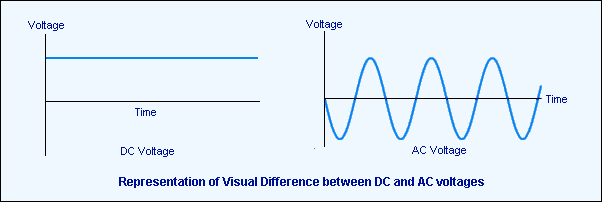
\includegraphics[width=0.8\textwidth]{res/acdc.png}
  \end{figure}

%   \begin{itemize}
%     \item
%       Converts AC in the walls, into DC for the computer.
%   \end{itemize}
\end{frame}

\section{Electricity}

\begin{frame}
  \frametitle{Electricity \& our first circuit}

  \begin{columns}
    \begin{column}{0.5\textwidth}
      \begin{center}
        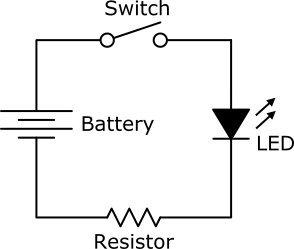
\includegraphics[width=\textwidth]{res/led-diagram.png}
      \end{center}
    \end{column}
    \begin{column}{0.5\textwidth}
      \begin{itemize}
        \item Current flows clockwise in this diagram.
        \item The battery generates direct current.
        \item We associate a positive voltage with \texttt{true} and the
          negative voltage with \texttt{false}: \emph{binary!}
        \item We can build this circuit on a \emph{breadboard.}
      \end{itemize}
    \end{column}
  \end{columns}
\end{frame}

\begin{frame}
  \frametitle{Keeping things aligned}
  \begin{columns}
    \begin{column}{0.5\textwidth}
      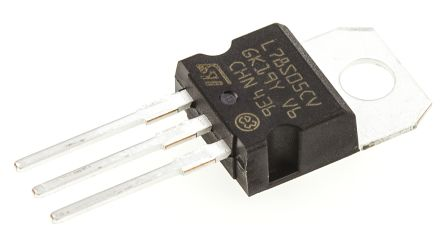
\includegraphics[width=\textwidth]{res/lvr.jpg}
    \end{column}
    \begin{column}{0.5\textwidth}
      \begin{itemize}
        \item
          The \emph{(linear) voltage regulator} lowers its input voltage to a
          fixed value.
        \item
          We use this to convert down from the 9~V battery to 5~V, which is
          closer to the range our other components are meant for.
      \end{itemize}
    \end{column}
  \end{columns}
\end{frame}

\begin{frame}
  \frametitle{Vive la resistance}

  \begin{columns}
    \begin{column}{0.5\textwidth}
      \centering
      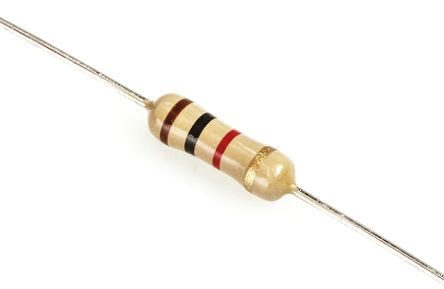
\includegraphics[width=0.8\textwidth]{res/resistor.jpg}

      ~ \\

      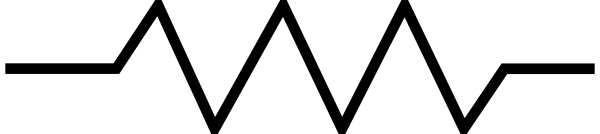
\includegraphics[width=0.8\textwidth]{res/resistor-symbol.png}
    \end{column}
    \begin{column}{0.5\textwidth}
      A resistor \emph{slows down} the current moving through it.

      We need this so that our light doesn't blow up!
    \end{column}
  \end{columns}
\end{frame}

\begin{frame}
  \frametitle{The light of my life}

  \begin{columns}
    \begin{column}{0.5\textwidth}
      \centering
      
      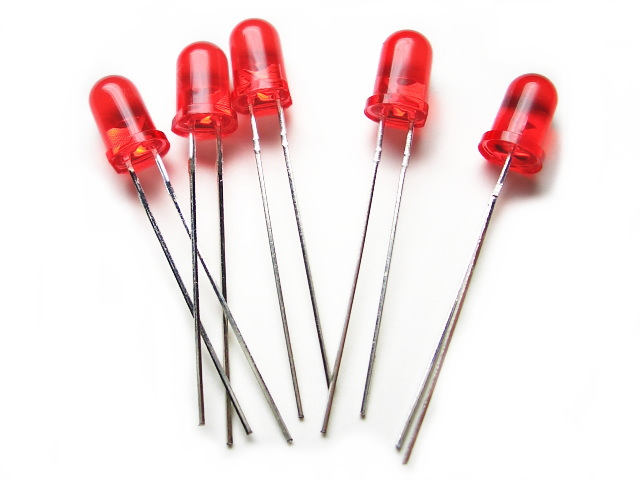
\includegraphics[width=0.6\textwidth]{res/led.jpg}

      ~ \\

      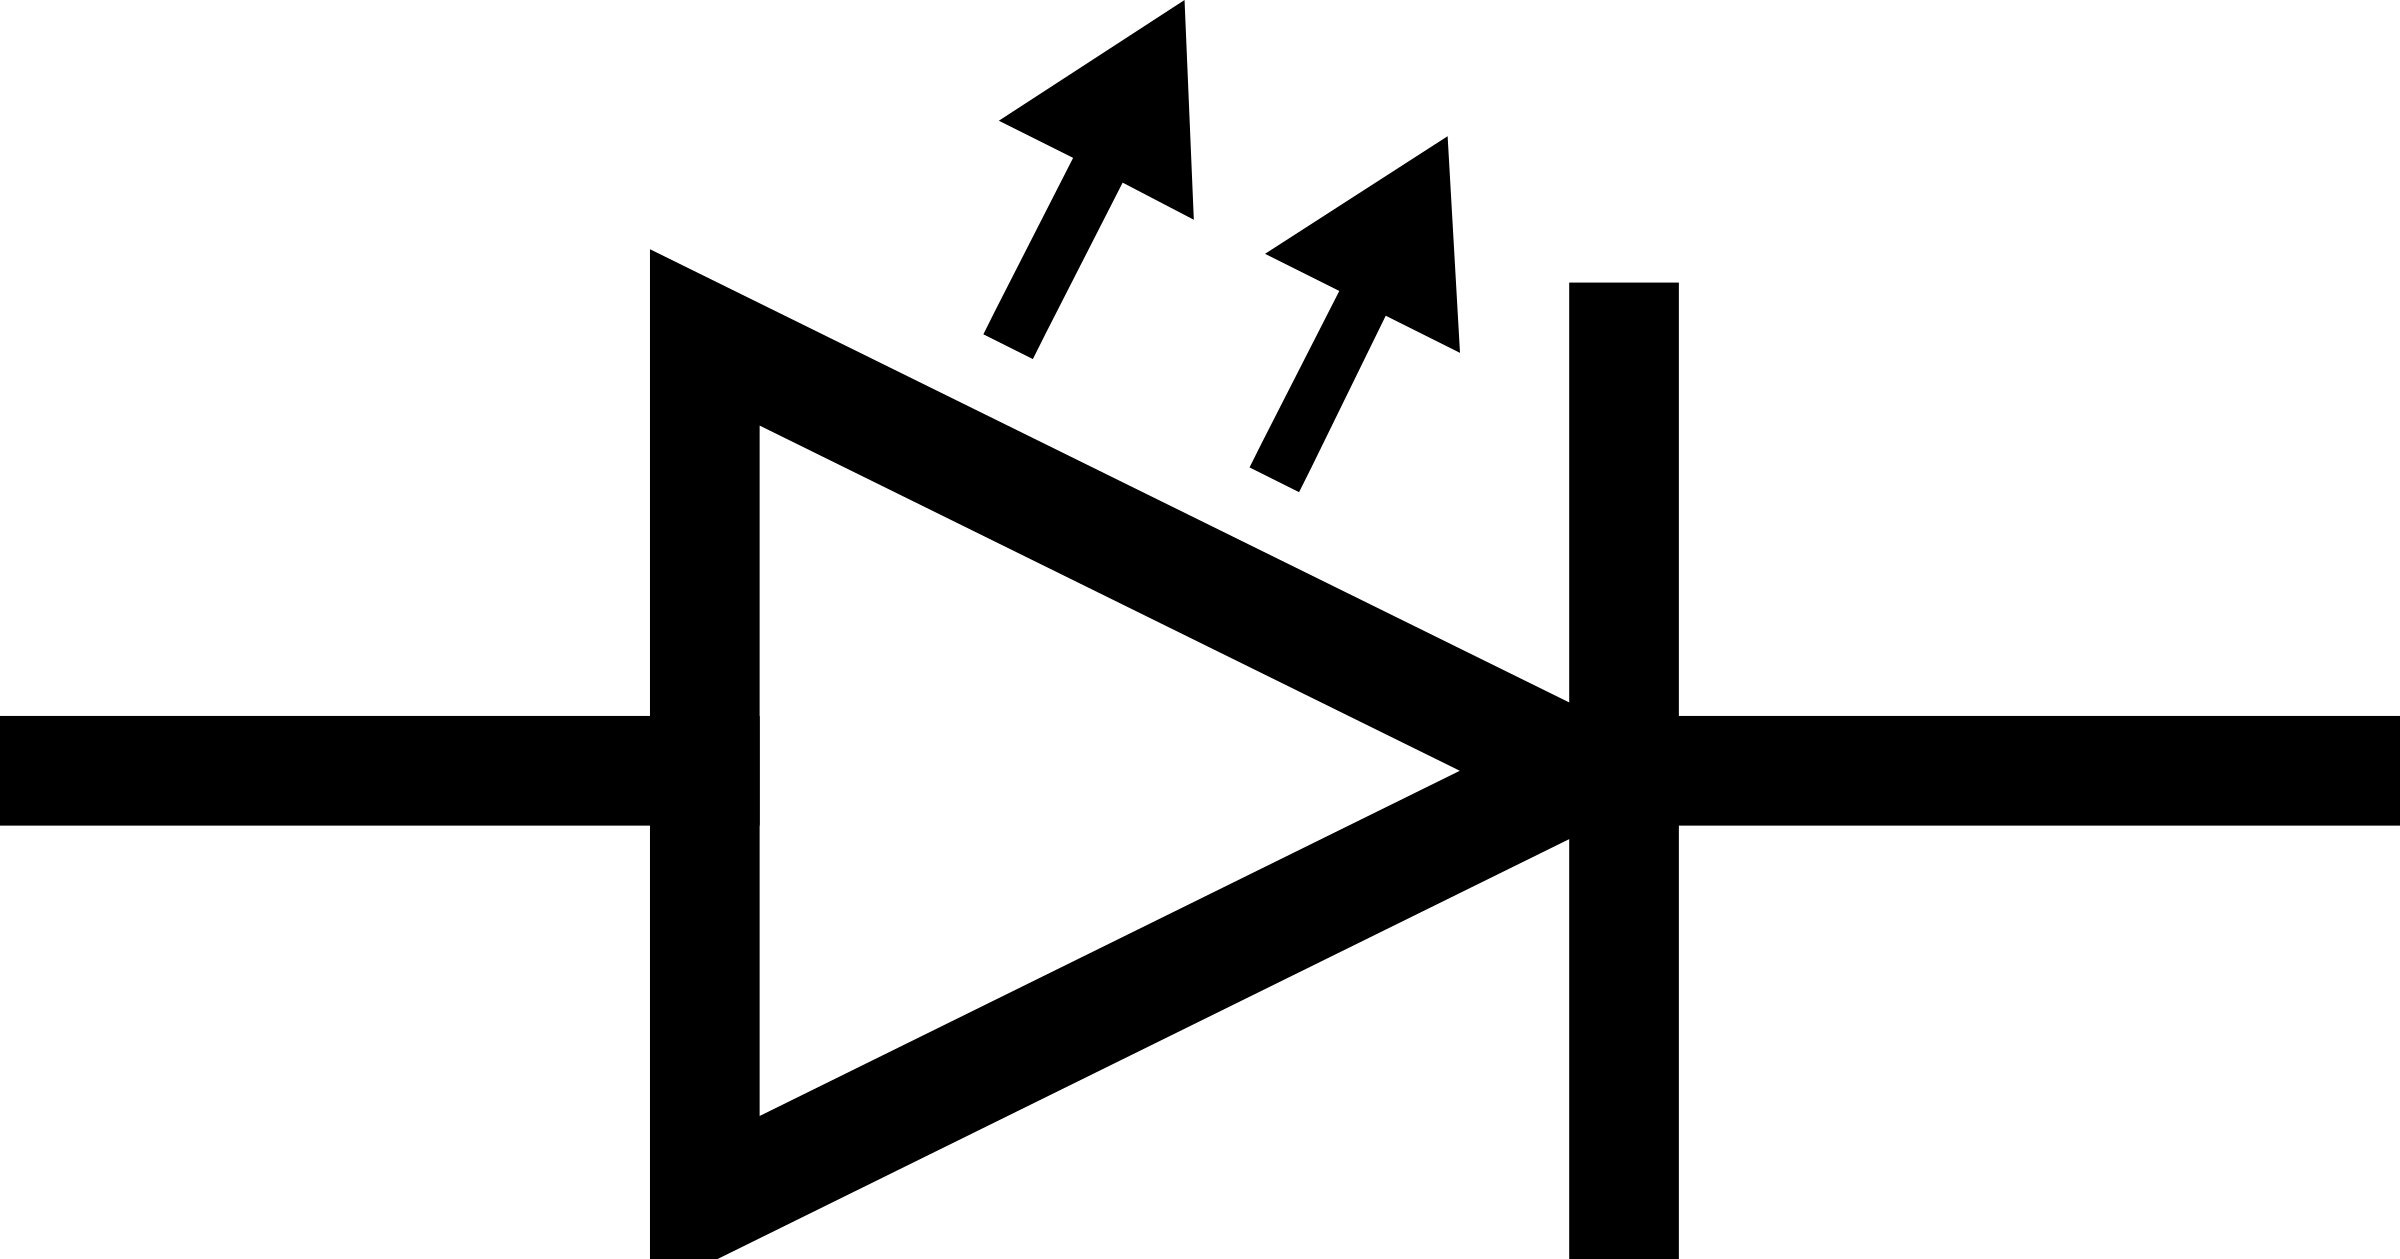
\includegraphics[width=0.6\textwidth]{res/led-symbol.png}
    \end{column}
    \begin{column}{0.5\textwidth}
      \begin{itemize}
        \item
          \emph{LED}s emit light when current passes through.
        \item
          LEDs have \emph{polarity}: the direction they're facing in the circuit
          makes a difference!
          (In contrast, resistors do not have polarity.)

        \item
          The long leg is the \emph{positive} terminal.
      \end{itemize}
    \end{column}
  \end{columns}
\end{frame}

\begin{frame}
  \frametitle{A board for cutting bread? Not really.}

  \begin{columns}
    \begin{column}{0.5\textwidth}
      \centering
      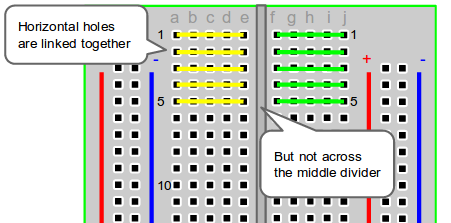
\includegraphics[width=\textwidth]{res/bb-diag.png}

      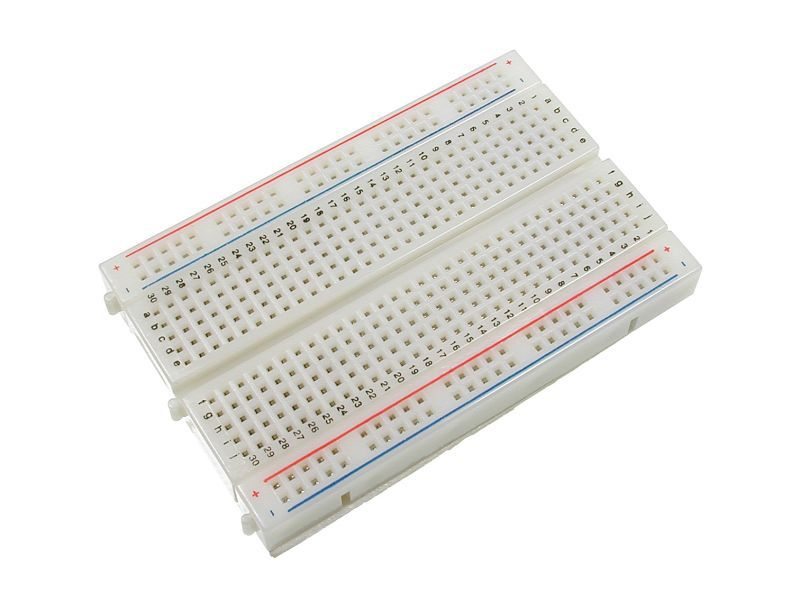
\includegraphics[width=\textwidth]{res/breadboard.jpg}
    \end{column}
    \begin{column}{0.5\textwidth}
      And the holes on the left and right, called \emph{rails}, are connected vertically.
    \end{column}
  \end{columns}
\end{frame}

\begin{frame}
  \frametitle{Last but not least}
  
  \begin{columns}
    \begin{column}{0.5\textwidth}
      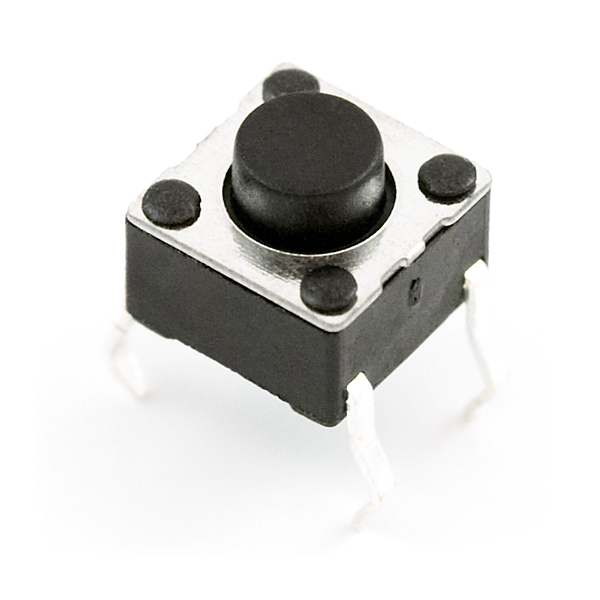
\includegraphics[width=\textwidth]{res/push-button.jpg}
    \end{column}
    \begin{column}{0.5\textwidth}
      \begin{itemize}
        \item
          In its neutral state, the button allows current to flow top-down
          through it.

        \item
          Pushing down on the button causes electricity to flow \emph{across} it.
      \end{itemize}
    \end{column}
  \end{columns}
\end{frame}

\begin{frame}
  \frametitle{Now let's build it!}
  \centering
  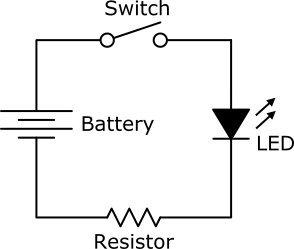
\includegraphics[width=0.5\textwidth]{res/led-diagram.png}
\end{frame}

\section{Electronic switches: transistors}

\begin{frame}
  \frametitle{Transistors: electronic switches}

  \begin{columns}
    \begin{column}{0.5\textwidth}
      \centering
      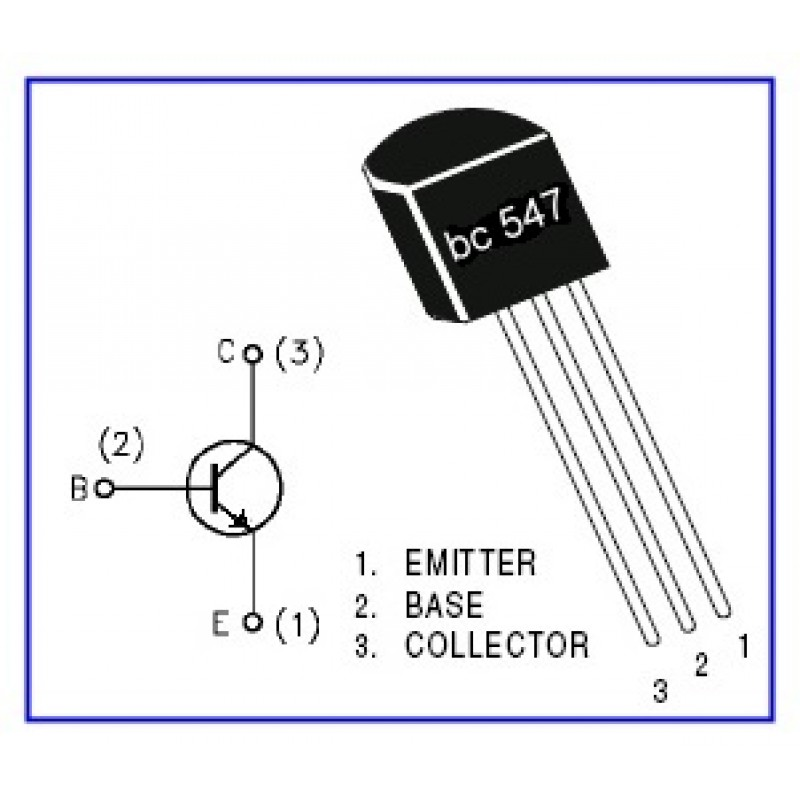
\includegraphics[width=\textwidth]{res/transistor.jpg}
    \end{column}
    \begin{column}{0.5\textwidth}
      \begin{itemize}
        \item
          When current is applied to the \emph{base} of the transistor, current
          is allowed to flow from the \emph{collector} to the \emph{emitter}.
        \item
          Transistors are the basic building blocks of more complex circuits,
          such as CPUs!
      \end{itemize}
    \end{column}
  \end{columns}
\end{frame}

\begin{frame}
  \frametitle{Now let's use a transistor!}
  Replace the switch with a transistor, and use the \emph{base} to control the LED.

  \begin{center}
    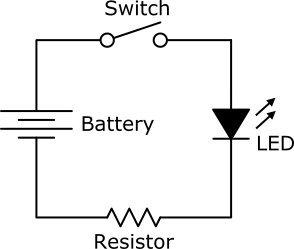
\includegraphics[width=0.5\textwidth]{res/led-diagram.png}
  \end{center}
\end{frame}

\section{Logic gates}

\begin{frame}
  \frametitle{Two transistors in series makes an AND gate}

  \begin{center}
    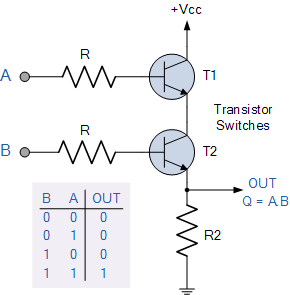
\includegraphics[width=0.55\textwidth]{res/and-transistor.png}
  \end{center}

  Try putting the LED both on the collector side and emitter side of the
  transistor pair.
\end{frame}

\begin{frame}
  \frametitle{Two transistors in parallel makes an OR gate}

  \begin{center}
    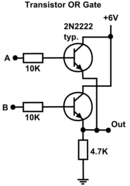
\includegraphics[width=0.4\textwidth]{res/or-gate.png}
  \end{center}
\end{frame}

\begin{frame}
  \frametitle{Recap}
  \tableofcontents
\end{frame}

\begin{frame}
  \frametitle{Homework}

  \begin{itemize}
    \item
      Check out \url{https://tryhaskell.org/}!

    \item
      Try getting to lesson 4.
  \end{itemize}
\end{frame}

\end{document}
